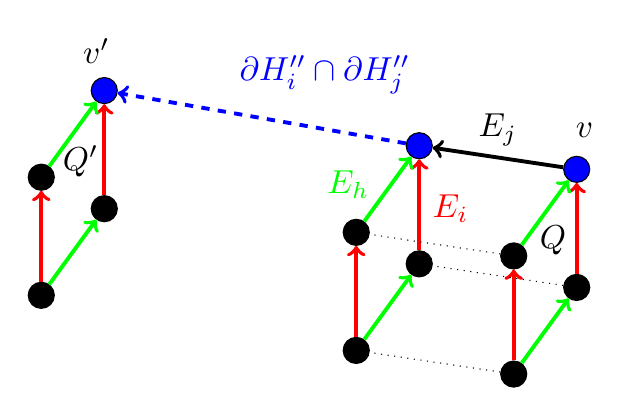
\begin{tikzpicture}

% NODES %%%%%%%%%%%%%%%%%%%%%%%%%%%%%%%%%%%%%%%%%%%%%%%%%%%%%%%%%%%%%%%%%%

\node[draw, circle, minimum height=0.2cm, minimum width=0.2cm, fill=blue] (P5) at (5.0,4.0) {};
\node[draw, circle, minimum height=0.2cm, minimum width=0.2cm, fill=black] (P5b) at (5.0,2.5) {};
\node[draw, circle, minimum height=0.2cm, minimum width=0.2cm, fill=black] (P5c) at (4.2,2.9) {};
\node[draw, circle, minimum height=0.2cm, minimum width=0.2cm, fill=black] (P5d) at (4.2,1.4) {};

%\node[draw, circle, minimum height=0.2cm, minimum width=0.2cm, fill=black] (P6) at (7.0,3.1) {};
%\node[draw, circle, minimum height=0.2cm, minimum width=0.2cm, fill=black] (P6b) at (7.0,1.6) {};

\node[draw, circle, minimum height=0.2cm, minimum width=0.2cm, fill=blue] (P7) at (9.0,3.3) {};
\node[draw, circle, minimum height=0.2cm, minimum width=0.2cm, fill=black] (P7b) at (9.0,1.8) {};
\node[draw, circle, minimum height=0.2cm, minimum width=0.2cm, fill=black] (P7c) at (8.2,2.2) {};
\node[draw, circle, minimum height=0.2cm, minimum width=0.2cm, fill=black] (P7d) at (8.2,0.7) {};

\node[draw, circle, minimum height=0.2cm, minimum width=0.2cm, fill=blue] (P8) at (11.0,3.0) {};
\node[draw, circle, minimum height=0.2cm, minimum width=0.2cm, fill=black] (P8b) at (11.0,1.5) {};
\node[draw, circle, minimum height=0.2cm, minimum width=0.2cm, fill=black] (P8c) at (10.2,1.9) {};
\node[draw, circle, minimum height=0.2cm, minimum width=0.2cm, fill=black] (P8d) at (10.2,0.4) {};


% LINKS %%%%%%%%%%%%%%%%%%%%%%%%%%%%%%%%%%%%%%%%%%%%%%%%%%%%%%%%%%%%%%%%%%


\draw[->,line width = 1.4pt, color = red] (P5b) -- (P5);
\draw[->,line width = 1.4pt, color = green] (P5c) -- (P5);
\draw[->,line width = 1.4pt, color = red] (P5d) -- (P5c);
\draw[->,line width = 1.4pt, color = green] (P5d) -- (P5b);

\draw[->,line width = 1.4pt, dashed, color = blue] (P7) -- (P5);

\draw[->,line width = 1.4pt, color = red] (P7b) -- (P7);
\draw[->,line width = 1.4pt, color = green] (P7c) -- (P7);
\draw[->,line width = 1.4pt, color = red] (P7d) -- (P7c);
\draw[->,line width = 1.4pt, color = green] (P7d) -- (P7b);

\draw[->,line width = 1.4pt] (P8) -- (P7);
\draw[->,line width = 1.4pt, color = red] (P8b) -- (P8);
\draw[->,line width = 1.4pt, color = green] (P8c) -- (P8);
\draw[->,line width = 1.4pt, color = red] (P8d) -- (P8c);
\draw[->,line width = 1.4pt, color = green] (P8d) -- (P8b);

\draw[dotted] (P8b) -- (P7b);
\draw[dotted] (P8c) -- (P7c);
\draw[dotted] (P8d) -- (P7d);

% ETIQUETTES

\node[scale=1.2, color = red] at (9.4,2.5) {$E_i$};
\node[scale=1.2, color = green] at (8.1,2.8) {$E_h$};
\node[scale=1.2, color = black] at (10.0,3.5) {$E_j$};

\node[scale = 1.2, color = blue] at (7.8,4.2) {$\partial H_i'' \cap \partial H_j''$};

\node[scale=1.2] at (4.9,4.5) {$v'$};
\node[scale=1.2] at (11.1,3.5) {$v$};

\node[scale=1.2] at (4.7,3.1) {$Q'$};
\node[scale=1.2] at (10.7,2.1) {$Q$};

\end{tikzpicture}